%
% File acl2019.tex
%
%% Based on the style files for ACL 2018, NAACL 2018/19, which were
%% Based on the style files for ACL-2015, with some improvements
%%  taken from the NAACL-2016 style
%% Based on the style files for ACL-2014, which were, in turn,
%% based on ACL-2013, ACL-2012, ACL-2011, ACL-2010, ACL-IJCNLP-2009,
%% EACL-2009, IJCNLP-2008...
%% Based on the style files for EACL 2006 by 
%%e.agirre@ehu.es or Sergi.Balari@uab.es
%% and that of ACL 08 by Joakim Nivre and Noah Smith

\documentclass[11pt,a4paper]{article}
\usepackage[hyperref]{acl2019}
\usepackage{times}
\usepackage{latexsym}
\usepackage{amsmath}
\usepackage{graphicx}
\usepackage{caption}
\usepackage{subcaption}
\DeclareMathOperator*{\argmax}{arg\,max}
\DeclareMathOperator*{\argmin}{arg\,min}

\usepackage{url}

\aclfinalcopy % Uncomment this line for the final submission
%\def\aclpaperid{***} %  Enter the acl Paper ID here

%\setlength\titlebox{5cm}
% You can expand the titlebox if you need extra space
% to show all the authors. Please do not make the titlebox
% smaller than 5cm (the original size); we will check this
% in the camera-ready version and ask you to change it back.
\newcommand\BibTeX{B\textsc{ib}\TeX}

\title{Concept Tagging for the Movie Domain}

\author{Giovanni De Toni (197814) \\
  University of Trento \\ Via Sommarive, 9, 38123 Povo,Trento TN\\
  \texttt{giovanni.detoni@studenti.unitn.it}}

\date{}

\begin{document}
\maketitle

\begin{abstract}
This work focuses on the well-known task of concept tagging phrase elements.
This present a relatively important challenge in the NLP field since it is
the starting point for more complex application. Weighted Finite State Transducer
and statistical method were used and an analysis of their performances is also provided.
\end{abstract}

\section{Introduction}
One of the first step of some NLP task is to analyze a given phrase to understand its underlying concept. For instance, imagine we are using a vocal application to order something to eat (e.g., "I would like a tortel di patate delivered at Piazza Trento 1, please"). In order for a machine to understand correctly what we want, firstly it needs to convert our utterances to a word representation, secondly it needs to assign concept to each of the word it heard (e.g., "tortel di patate" equals to requested food and "Piazza Trento 1" equals to the delivery address).
This basic operation is of utmost importance for all the application which can be built upon this. For instance, the quality of you food assistant is dependent on the quality of this concept tagger. Imagine what could happen if the machine were to swap the delivery address with the requested food!).  
The scope of this project is to provide a simple concept-tagger by developing a WSTF (Weighted Finite State Transducer) applied to the movie domain.
The report is detailed as follow: in the first section we define more formally the problem statement, then we proceed with an analysis of the given dataset and with the description of the models employed. Ultimately, we discuss the obtained results while underlying their stengths and limitations. 

\section{Problem Statement}
Given a sequence of tokens $<t_1, \ldots, t_n>$ and given a pool of concepts $<c_1, \ldots, c_m>$, we want to find the most likely assignment $<t_i, c_i>$ such that it maximizes the following probability:
\begin{equation*}
c_1, \ldots, c_n = \argmax_{c_1, \ldots, c_n} P (c_1, \ldots, c_n | t_1, \ldots, t_n)
\end{equation*}
Thanks to the Markov assumption (the probability of the $i$-th concept depends only on the $(i-1)$-th concept and the probability of the $i$-th token depends only on the $i$-th concept), we can simplify the previous formula. Moreover, we can also compute its component by MLE (Maximum Likelihood Estimation):
\begin{equation*}
c_1, \ldots, c_n = \argmax_{c_1, \ldots, c_n} P(t_i|c_i)P(c_i| c_{i-1})
\end{equation*}
In the previous formula, $P(t_i|c_i) = \frac{C(c_i, t_i)}{C(c_i)}$ and $P(c_i|c_{i-1}) = \frac{C(c_{i-1}, c_i)}{C(c_i)}$ (where $C(x)$ counts the occurrences of $x$ inside the given dataset). 

\section{Data Analysis}
The dataset used is called NL2SparQL4NLU. This work used only the "*.conll.txt" files (more specifically, one for training the language model and one for testing it). Each file is written using the token-per-line CONLL format with tokens and NLU concept tags. An analysis of the content of the two files follows:
\begin{table}[h]
\centering
\begin{tabular}{|l|l|}
\hline
\multicolumn{2}{|l|}{\textbf{NL2SparQL4NLU.trai.conll.txt}} \\ \hline
\textit{\# of lines}									& 24791 \\ \hline
\textit{\# of sentences}                             & 3338 \\ \hline
\textit{\# of unique tokens}                         & 1728 \\ \hline
\textit{\# of unique concepts (without the prefix)}  & 24   \\ \hline
\end{tabular}
\caption{Description of the content of the train dataset.}
\label{tab:train-dataset-description}
\end{table} 

\begin{table}[h]
\centering
\begin{tabular}{|l|l|}
\hline
\multicolumn{2}{|l|}{\textbf{NL2SparQL4NLU.test.conll.txt}} \\ \hline
\textit{\# of lines}									& 8201 \\ \hline
\textit{\# of sentences}                             & 1084 \\ \hline
\textit{\# of unique tokens}                         & 1039 \\ \hline
\textit{\# of unique concepts (without the prefix)}  & 23   \\ \hline
\end{tabular}
\caption{Description of the content of the test dataset.}
\label{tab:test-dataset-description}
\end{table} 

The distribution of the tokens was analyzed. It was found to behave accordingly to the
Zipf's Law, however, for brevity, it was not reported here since it was not showing 
anything interesting. The OOV rate for the tokens is around $23.68\%$. There are also
some tokens which are the results of mispelling (e.g., "dispaly", "Scorcese").
The distribution of the various concepts was also analyzed (both for the training
and the test datasets). The distribution of the various concepts is shown in Figure X.

\begin{figure}[t]
	\begin{subfigure}[b]{0.5\textwidth}
		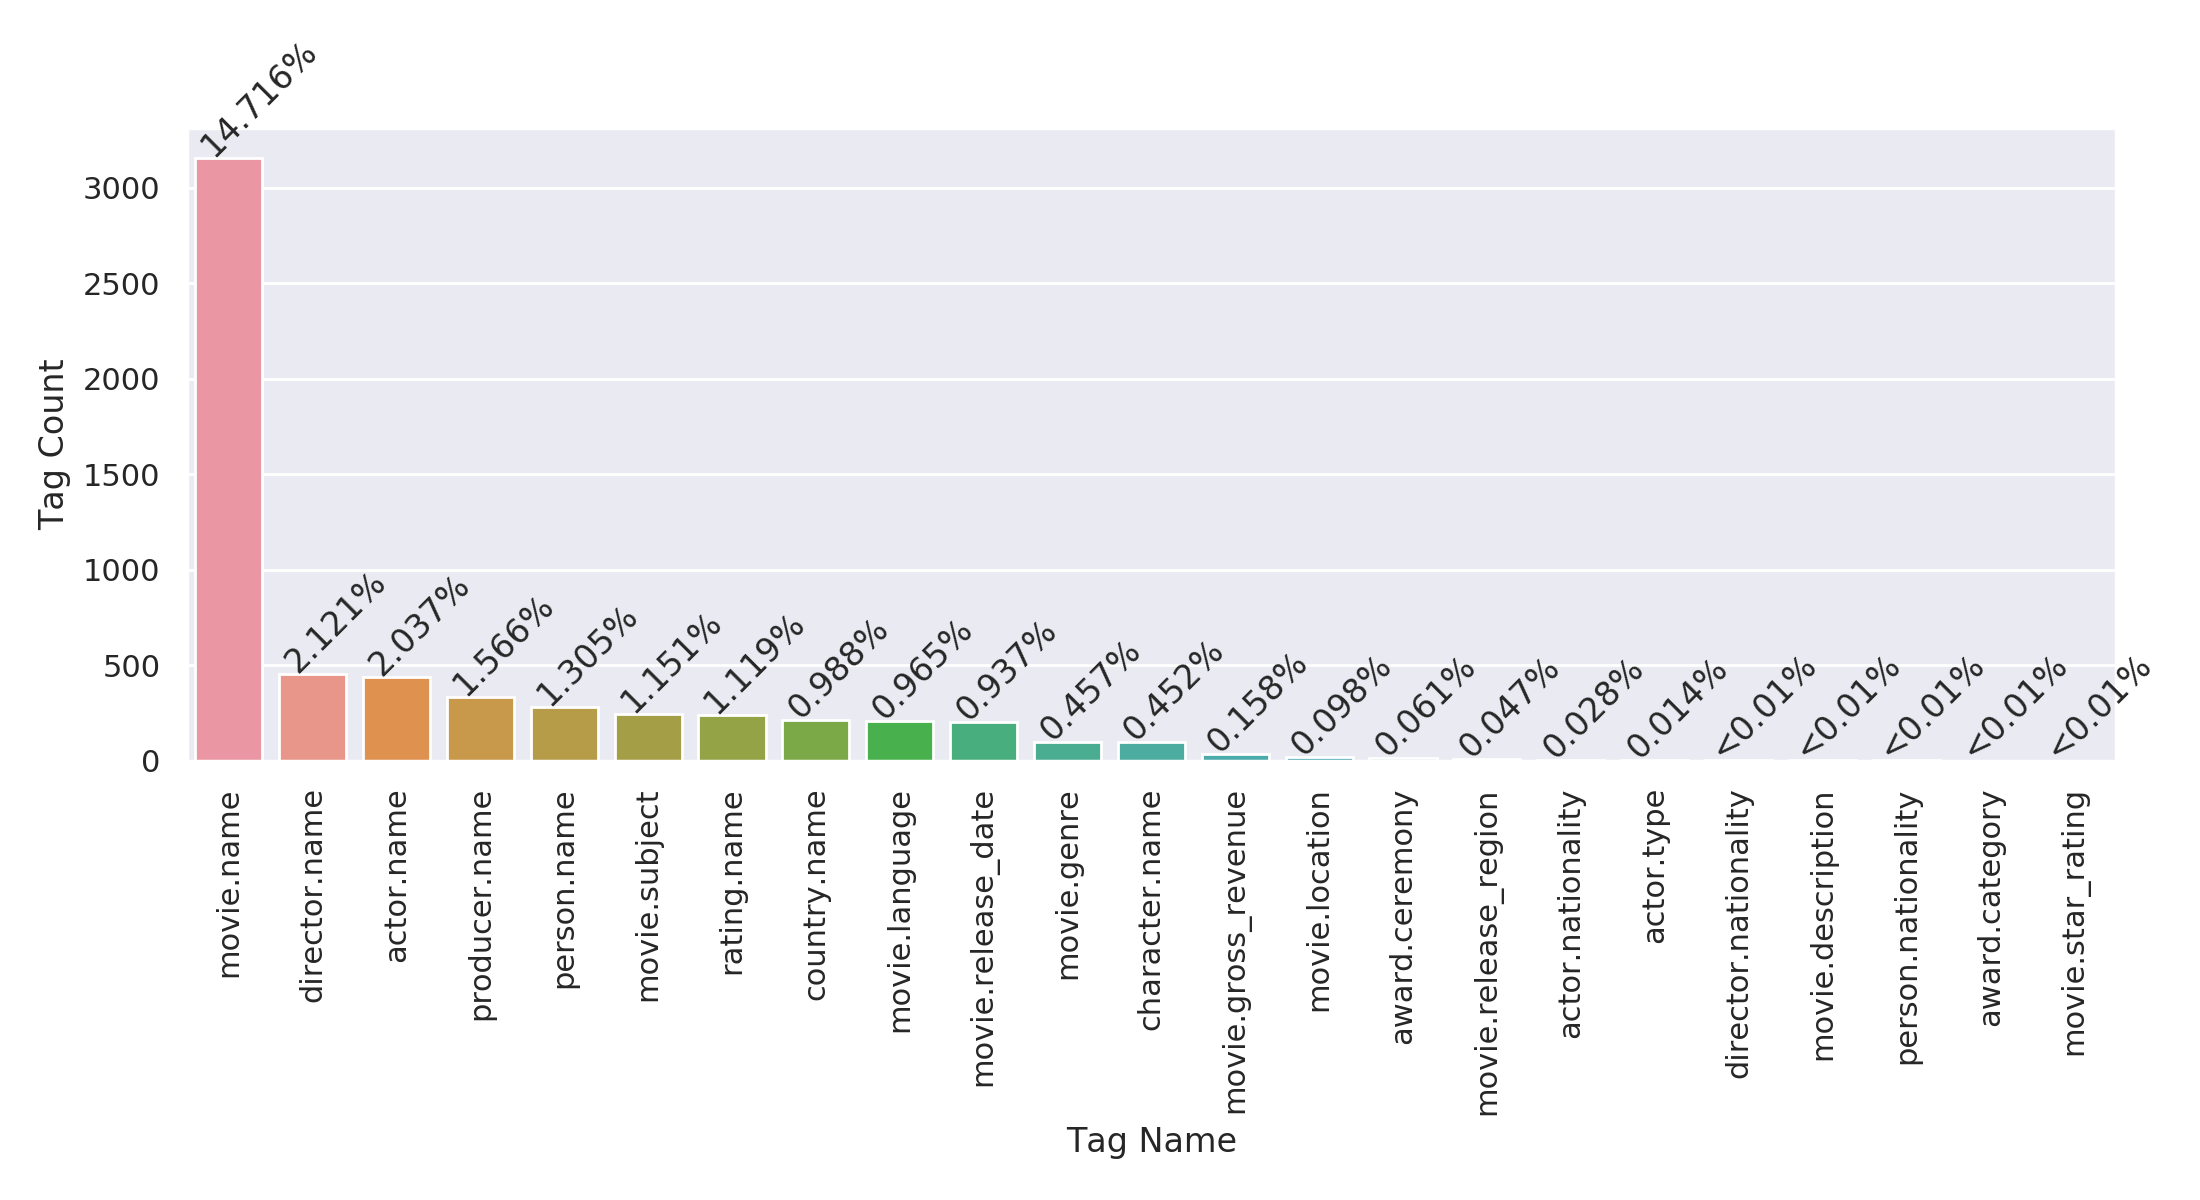
\includegraphics[width=\textwidth]{img/train-concepts-distribution}
		\caption{Train dataset.}
	\end{subfigure}
	\hfill
	\begin{subfigure}[b]{0.5\textwidth}
	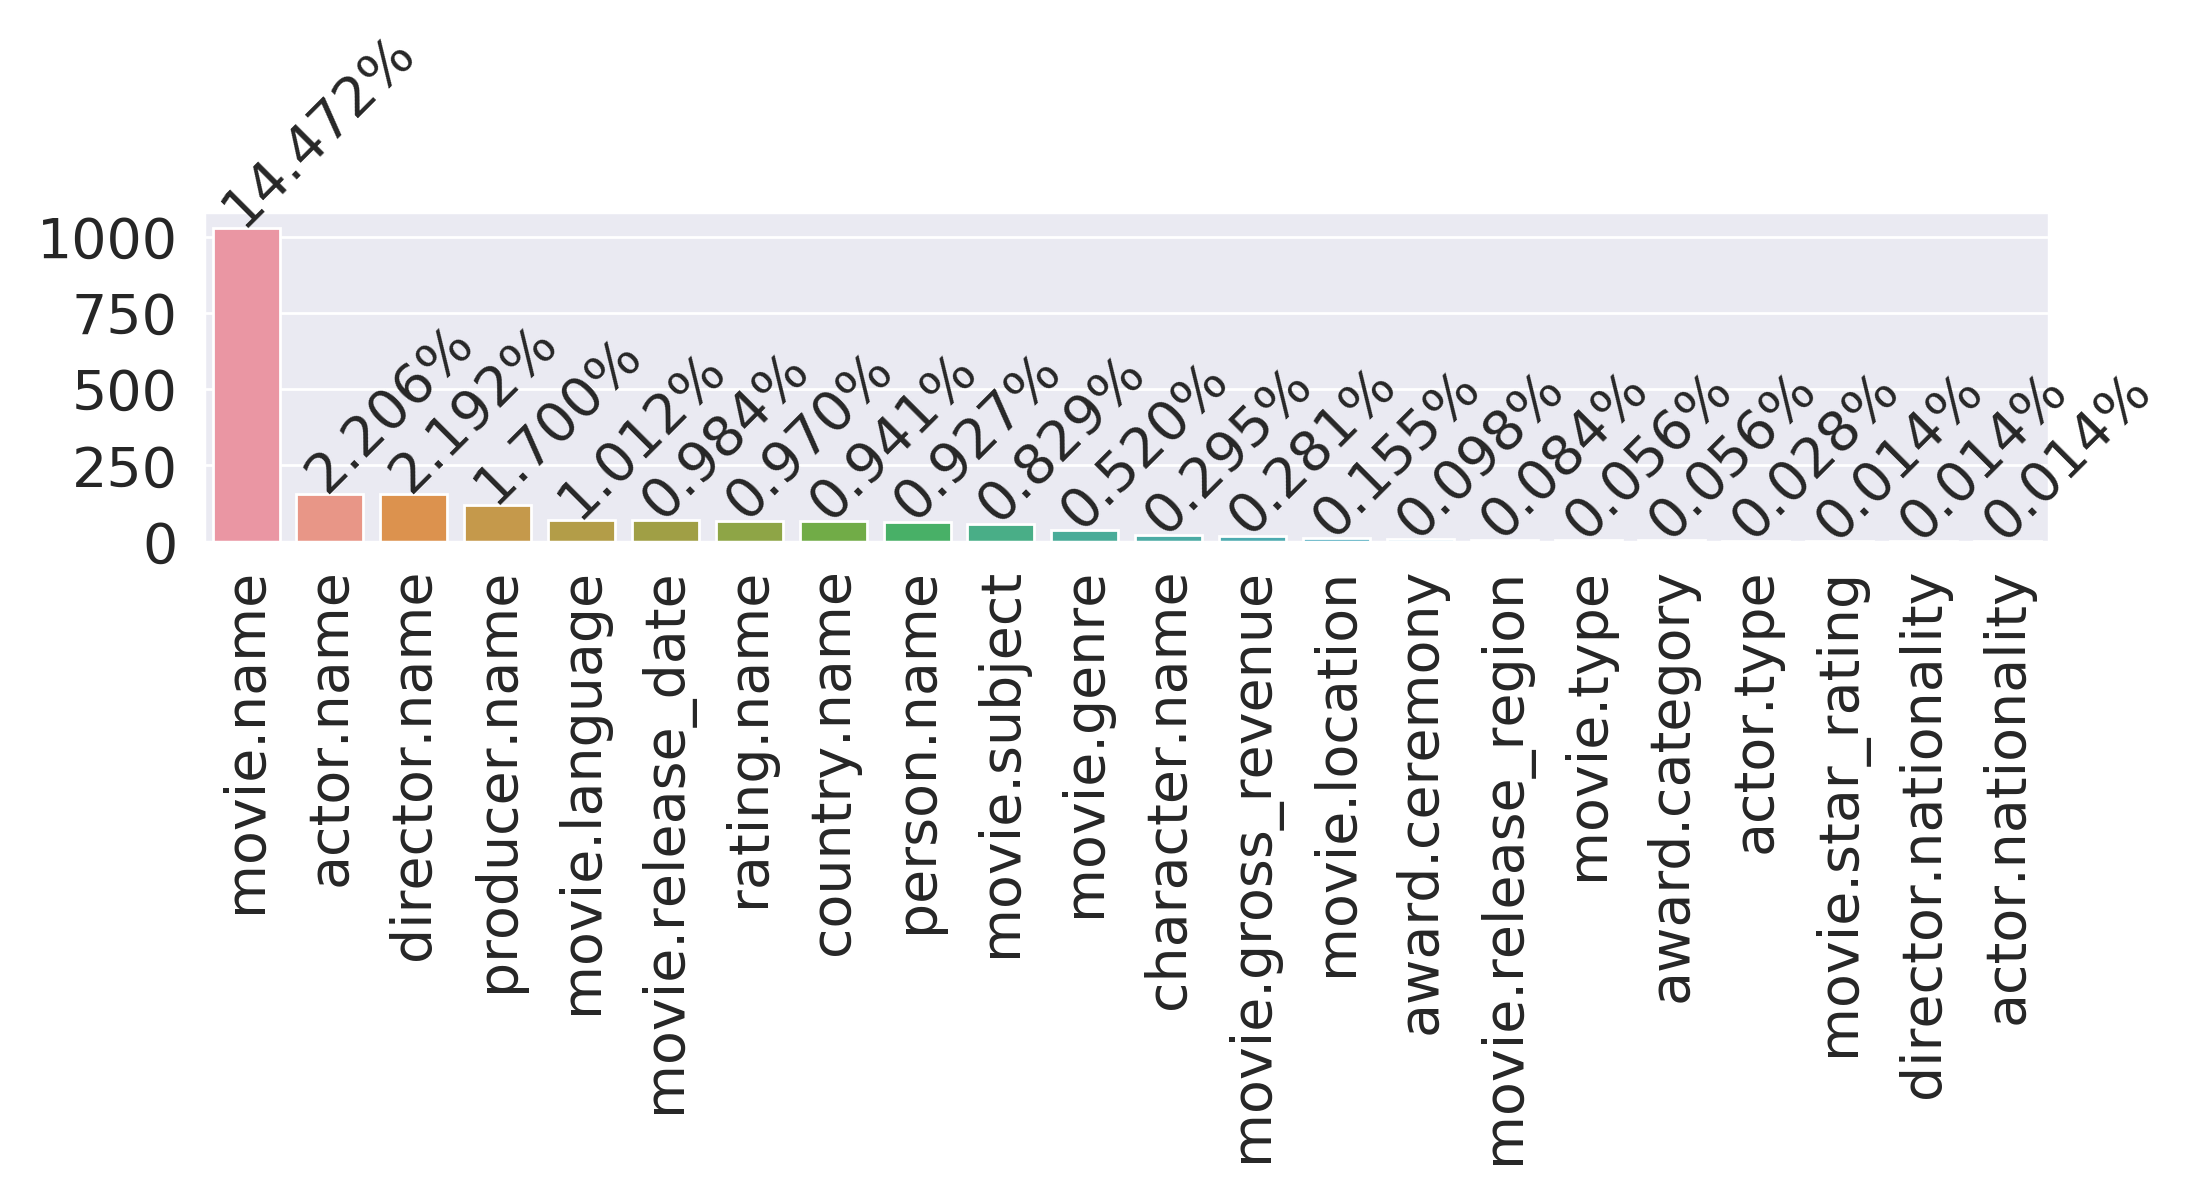
\includegraphics[width=\textwidth]{img/test-concepts-distribution}
	\caption{Test dataset.}
	\end{subfigure}
	\caption{Distributions of the various concepts in the train and test datasets. The \textit{O} was removed to make it easier to understand the weight of the others.}
\end{figure}


\section{Models}

\section{Experiments}

\section{Results}

\section{Credits}

\end{document}